% TeX root=../main.tex

\section{Descobrindo o luvita}

\emph{Luvita} denota um povo e uma língua e seus dialetos cuja existência,
até o começo do século passado, estava perdida na história.\footnote{Esta seção
	está baseada sobretudo em \textcite{CHLI11,Melchert2003,Hoffner2008}.}
Quando no final do século \textsc{xix} foram encontrados blocos de pedra no
norte da Síria com inscrições em hieroglifos em alto relevo, associaram esta
nova língua e o povo que a escreveu com os \emph{hititas}, um povo que até
então era lembrado por passagens da bíblia hebraica e alguns documentos
recentemente descobertos em assírio.
Em 1906, as escavações realizadas em Boğazköy\slash{}Boğazkale sob direção de
Hugo Winckler e Theodore Makridi revelaram a cidade de Hattusa,
capital do que teria sido depois chamado de Império Hitita, e nela um grande
arquivo de documentos em cuneiforme em uma língua até então
desconhecida.\footnote{A decifração do cuneiforme nesta altura já estava
	bastante adiantada, tendo sido iniciada nos primeiros anos do século
	\textsc{xix} e relativamente bem estabelecida dentro da primeira metade do
	século para o persa antigo, acadiano e elamita.}
Apenas em 1915-17, Bedřich Hrozný conseguiria ao mesmo tempo demonstrar que a
língua nesses arquivos e em duas cartas previamente escavadas em
\href{https://pleiades.stoa.org/places/149576487}{Tell el-Amarna}
(Egito moderno) era uma língua indo-europeia e produzir um esboço gramatical
dela, identificando-a como a língua dos hititas.
Entre os textos em cuneiforme escavados em Boğazköy entre 1906 e 22 revelaram
dentro deles trechos que os autores das tabuletas avisam que devem ser lidos
\emph{luwili}, isto é ``como luvita''.\footnote{Os códigos legais hititas
	contém provisões também de uma região, ainda hoje
com localização disputada, chamada \mbox{\textsc{kur} \textit{Lu-ú-i-ya}}.}
Como alguns termos soltos ou incluídos em léxicos dessa língua
aparecem marcados com um sinal cuneiforme, \foreignlanguage{hittite}{𒃵}, chamado
pelo nome alemão \emph{Glossenkeil}, sugeriu-se chamar essa língua também de
\emph{Glossenkeilsprache}.\footnote{Os textos em luvita cuneiforme estão
	editados em~\textcites{Starke1985}{YakubovichMouton2023}.
	Outra língua aparece, embora raramente, 
	nos textos hititas precedida por \foreignlanguage{hittite}{𒃵}, o palaico. Os
textos em palaico estão editados em~\textcite{Carruba1970}.}

A língua dos hieróglifos das inscrições sírias, no entanto, permaneceu
praticamente ilegível desde sua descoberta até a década de 30.\footnote{Alguns
	sinais tinham sido corretamente interpretados por Sayce entre 1882 e 1884, a
	saber os logogramas \mbox{L.17 𔐑 \textsc{rex}} e \mbox{L.228 𔔆 \textsc{regio}},
	respectivamente correspondentes aos cuneiformes
	\mbox{\foreignlanguage{hittite}{𒈗} \textsc{lugal}} `rei' e \mbox{\foreignlanguage{hittite}{𒆳} \textsc{kur}}
	`país\slash{}território'.}
No começo da década de 30, contribuições separadas de Meriggi, Gelb, Forrer,
Bossert e Hrozný ofereceram interpretação de diversos logogramas e
interpretações ou, ao menos, aproximações para alguns silabogramas,
permitindo as primeiras tentativas de interpretação.
Alguns avanços foram feitos durante as décadas de 1940 a 1960, com a compilação
de selos digráficos (hieroglíficos e cuneiformes) e com a publicação parcial da
inscrição bilíngue em hieroglífico e fenício de Karatepe descoberta por
Bossert e Halet Çambel.
Foi apenas com a publicação das ``Novas leituras''
por~\textcite{HawkinsMorpurgoNeumann1974} que se pode finalmente identificar a
língua dos hieróglifos hititas com a língua dos
\emph{\foreignlanguage{german}{Glossenkeil}} que deveriam
ser lidos \emph{luwili}.
Daí em diante, estas línguas passaram a ser conhecidas respectivamente como
\emph{luvita hieroglífico} e \emph{luvita cuneiforme}.

\section{Quando, onde, quem?}

Embora tenhamos contado um pouco sobre a descoberta e decifração do luvita
hieroglífico, convém dizer um pouco sobre o contexto histórico dessa língua.

\paragraph{Datação} Os primeiros textos legais hititas contendo menções à
terra chamada de \emph{Luwiya}, hit.\ \mbox{\textsc{kur} \textit{Lu-ú-i-ya}},
posteriormente chamada de Arzawa, datam da metade do segundo milênio antes da 
era comum, no Antigo Império Hitita.\footnote{CTH 291 e 292. Tradução das leis 
em \textcite{Hoffner1997}.}


\begin{compactenum}
\item Imperial: séc.\ \textsc{xiii aec}, entre as dinastias de Tudhaliya IV e
Suppiluliuma II
\item Neo-hitita: \emph{circa} 1100-700 \textsc{aec}
\end{compactenum}

\begin{figure}[ht!]
\begin{center}
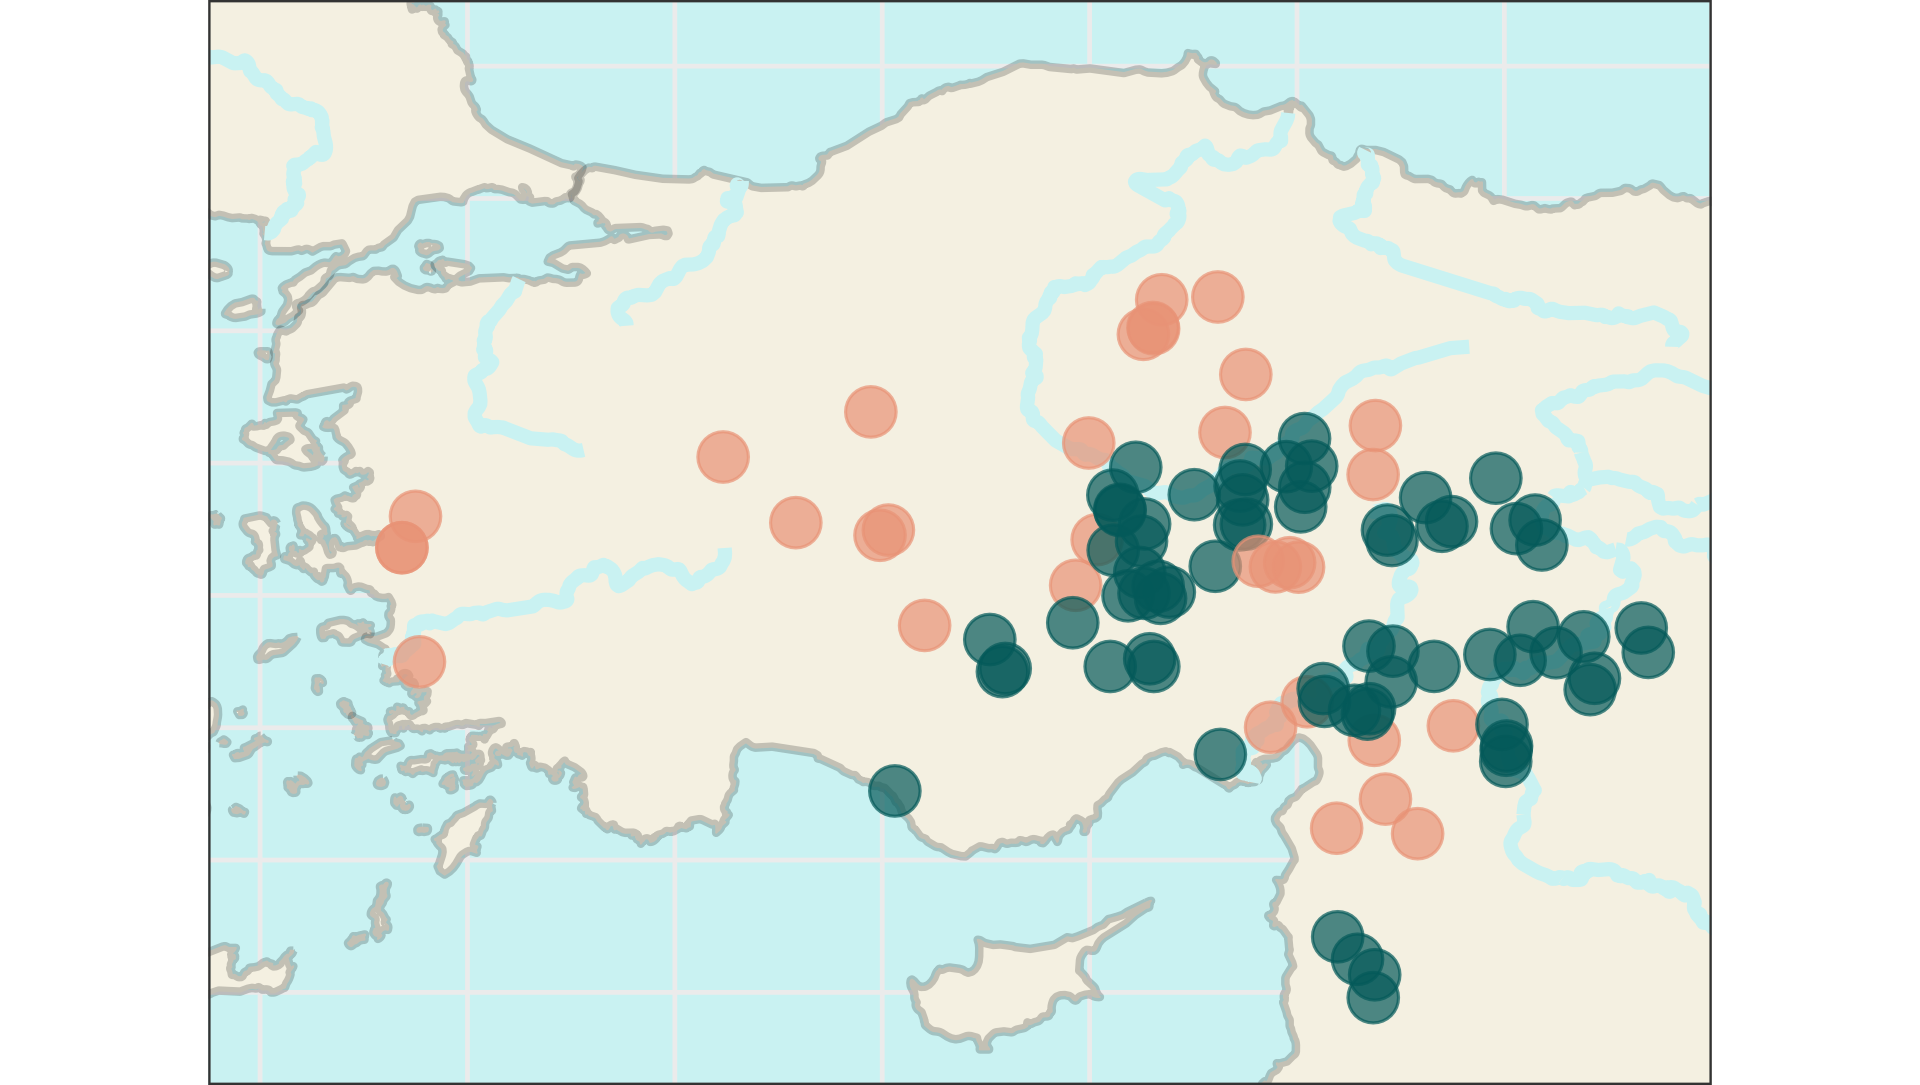
\includegraphics[width=1\textwidth]{../../Mídia/Map01.png}
\end{center}
\caption{Mapa contendo a localização das inscrições monumentais em luvita
hieroglífico. Os pontos laranjas representam inscrições do período imperial
enquanto os verdes, inscrições do período neo-hitita.}%\label{fig:mapa1}
\end{figure}
